\begingroup
\setlength{\unitlength}{0.01\columnwidth}
\begin{picture}(100,68.60)
  \put(0,0){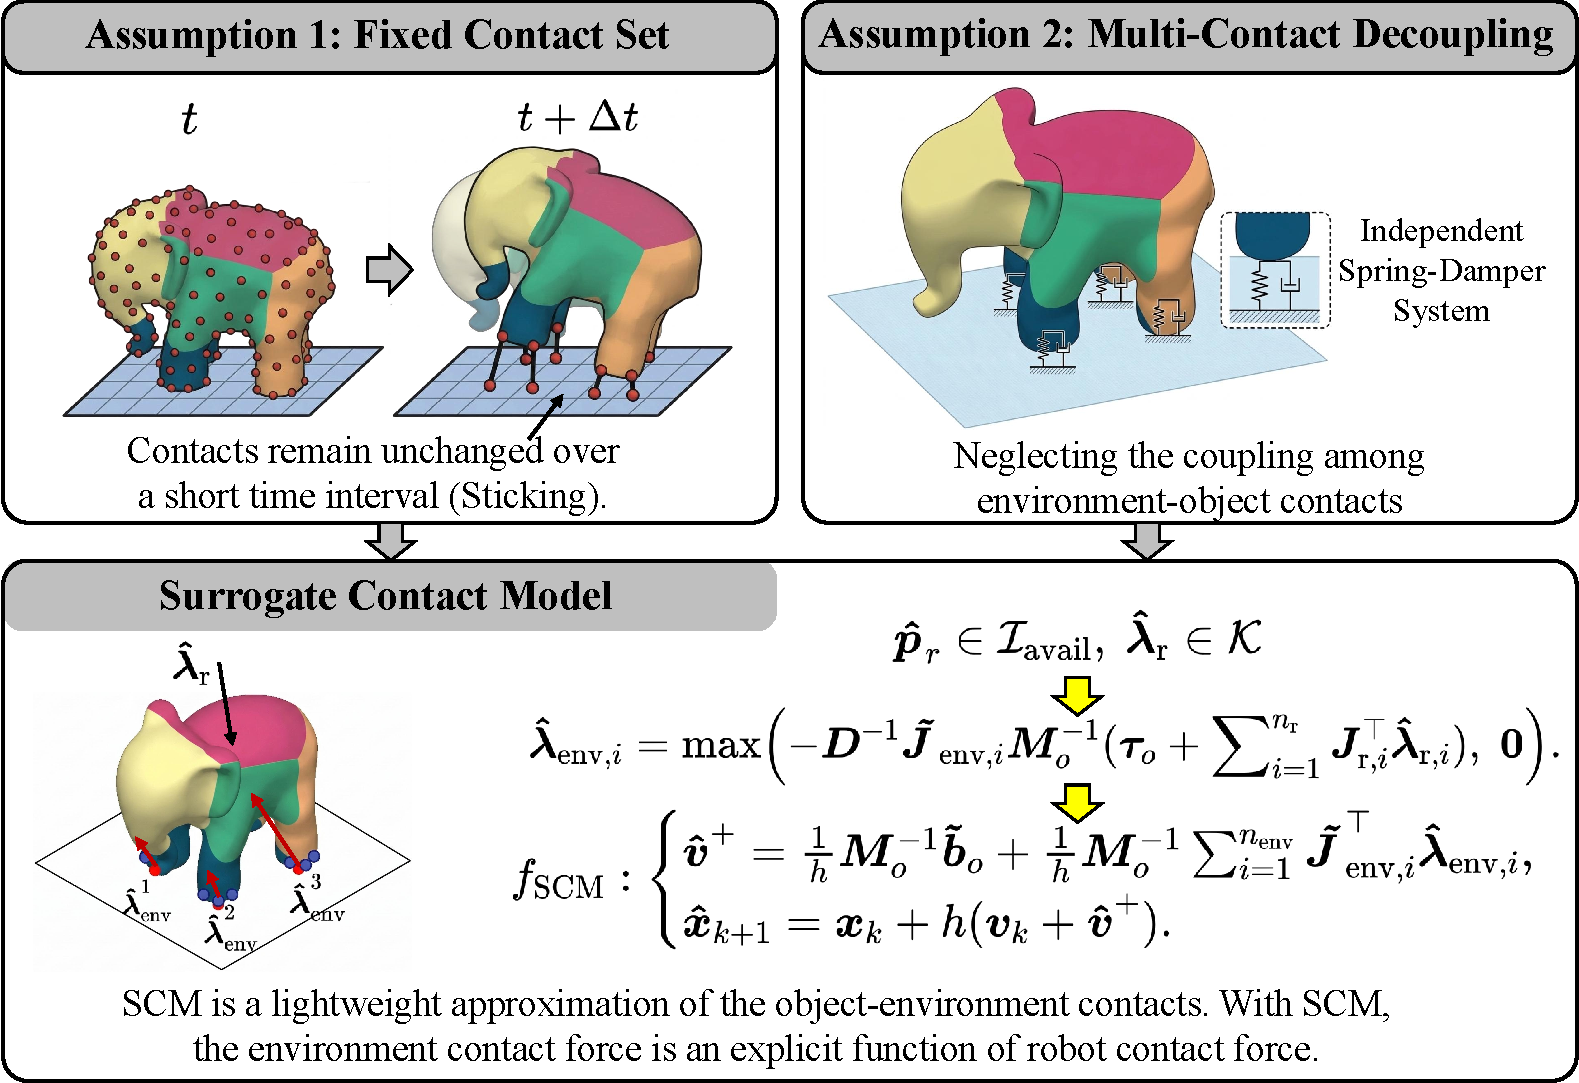
\includegraphics[width=\columnwidth]{figures/surrogate_contact_model.pdf}}
  \put(31,7.5){\color{white}\rule{0.68\columnwidth}{0.185\columnwidth}}
  \put(65,25.5){\vector(0,-1){2}}
  \put(32,20.5){\makebox(66,0){\fontsize{7}{8}\selectfont
    $\hat{\boldsymbol{\beta}}_{\mathrm{env},i}
    =\max\!\left[-\boldsymbol{D}^{-1}
    (a\boldsymbol{\tilde J}_{\mathrm{env},i}\boldsymbol{v}_{\mathrm{free}}
    +b\boldsymbol{\tilde\phi}_i/h),\boldsymbol{0}\right]$}}
  \put(65,18.5){\vector(0,-1){2}}
  \put(32,13.5){\makebox(66,0){\fontsize{7}{8}\selectfont
    $\hat{\boldsymbol{v}}^+=\boldsymbol{v}_{\mathrm{free}}
    +\boldsymbol{M}_o^{-1}\sum_i\boldsymbol{\tilde J}_{\mathrm{env},i}^{\top}
    \hat{\boldsymbol{\beta}}_{\mathrm{env},i}$}}
  \put(32,8.5){\makebox(66,0){\fontsize{7}{8}\selectfont
    $\hat{\boldsymbol{x}}_{k+1}=\boldsymbol{x}_k+h\hat{\boldsymbol{v}}^+$}}
\end{picture}
\endgroup
